%!TEX root = ../thesis.tex
% **************************** Define Graphics Path **************************
\ifpdf
\graphicspath{{Chapter5/Figs/Raster/}{Chapter5/Figs/PDF/}{Chapter5/Figs/}}
\else
\graphicspath{{Chapter5/Figs/Vector/}{Chapter5/Figs/}}
\fi

%*******************************************************************************
%****************************** Fifth Chapter *********************************
%*******************************************************************************

\chapter{Experiments and Results}
\label{chapter5}
In the penultimate chapter we present results obtained using the methodology and software presented in Chapter~\ref{chapter4}. We begin by discussing the training of rates $\Gamma^{(v)}$ and problems that we run into, before turning our attention to sampling with the obtained rates.  

\section{Training the rates}
\label{sec:training_exp}

\subsection{The elusive timescale $\lambda$}
\label{subsec:elusive_lambda}
An intuitive explanation of the Todorov loss introduced in section~\ref{subsec:todorov}, is in terms of penalisation for deviations away from the passive dynamics of the system, i.e. an agent has full control over the system but pays for straying far from the passive dynamics. Our method in its most basic form, using the \emph{latest} variational rates $\Gamma^{(v)}_{s \rightarrow s^\prime}$ to sample and using \emph{permute} batch generation, seems to completely disregard this penalty for straying far away from the passive dynamics when applied to the TFIM. Optimised rates $\Gamma_*^{(v)}$ obtained with this method vary depending on the initialisation, but the training itself is not sensitive to it. It is robust in the sense that low loss is obtained irrespective of the initialisation, barring vary bad hyperparameter settings, but the rates $\Gamma_*^{(v_i)}$ corresponding to these low losses are not the same. At first glance it appears that there are many \emph{local optima} for the rates, or alternatively, that there is an invariance in the loss and many rates are optimal. The latter turns out to be true. We refer to this problem as the inability to learn the correct \textbf{timescale} $\lambda$. This issue is illustrated in Fig.~\ref{fig:scaleblowup} which shows the number of spin flips in the sampled trajectory throughout training for three initialisations, along with the distributions of holding times $P \sim \tau$ of the final learned rates.
\begin{figure}[t]
	\centering
	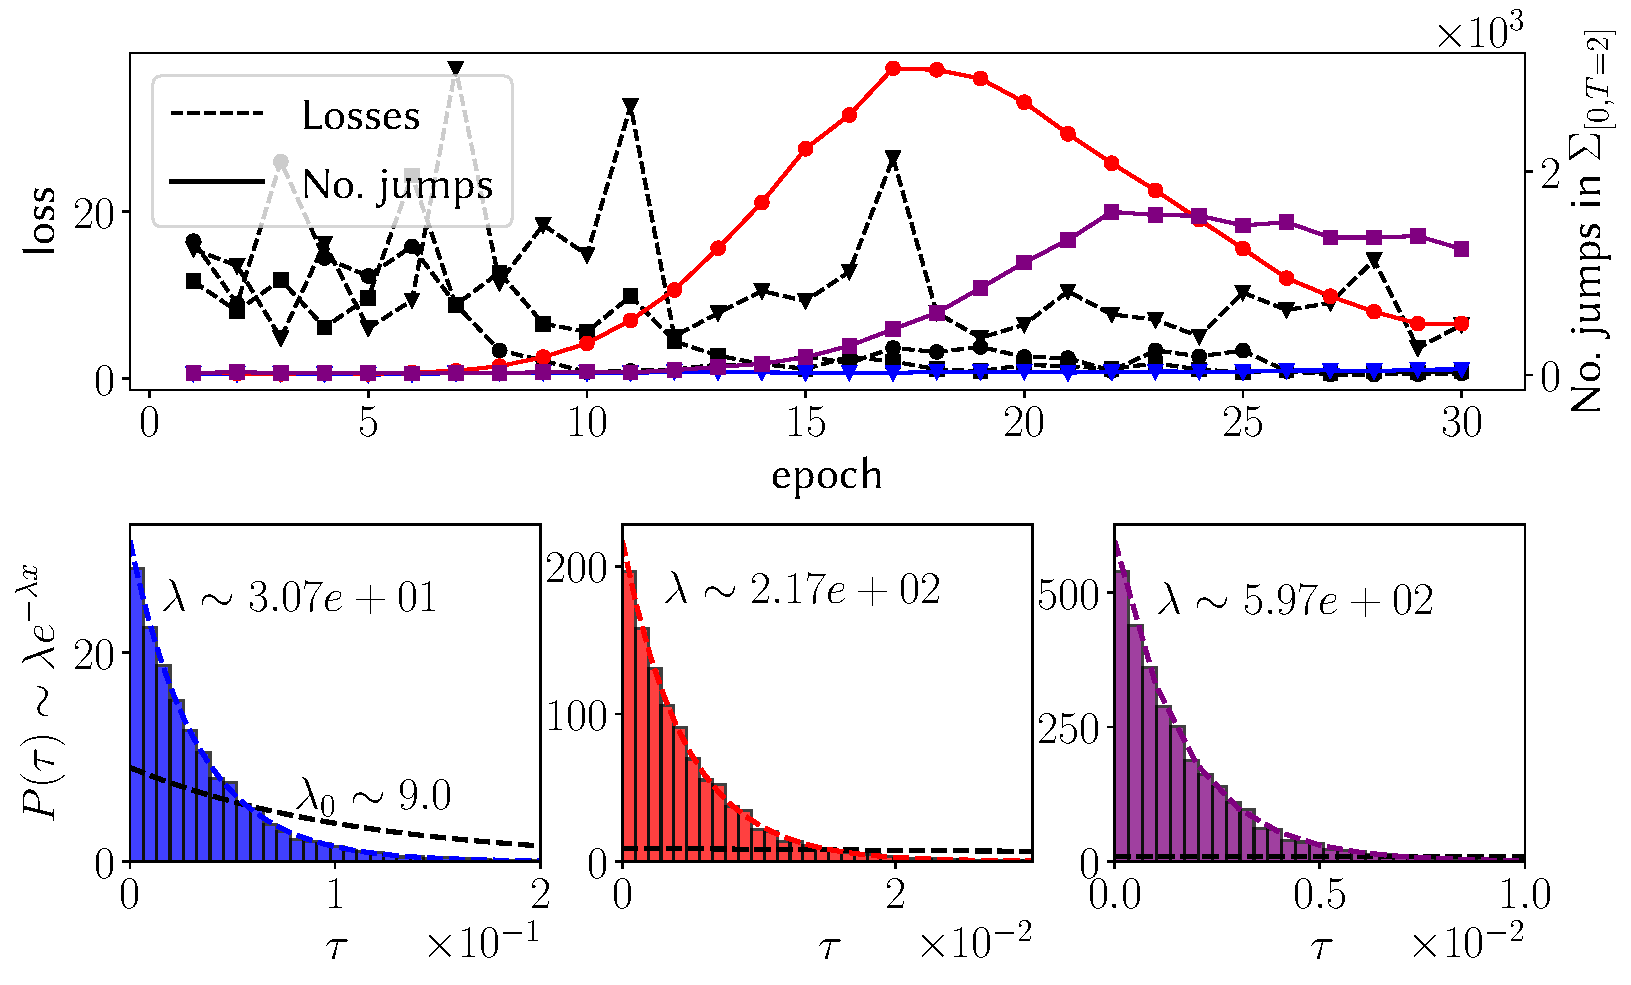
\includegraphics[width=\linewidth]{Chapter5/Figs/Vector/scale_blowup}
	\caption[The inability of the method to learn the correct timescale $\lambda$]{\textbf{The inability of the method to learn the correct timescale $\lambda$.} The $\log \text{RN}$ + \emph{permute} batch, fails to learn the correct timescale of the TFIM model. Figure shows the discrepancy between three learned rates in 1D ($L=8, J=1.0, g=1.0$). We see that the number of flips in the original sampled trajectory varies wildly throughout training, and is not related to the loss (\textbf{top}). All three initialisations reach low loss, but corresponding learned rates vary in scale, as exemplified by the distribution of holding times $\tau_i$ of each CTMC (\textbf{bottom}). The rate parameter $\lambda$ can be orders of magnitude different from the passive rates $\lambda_0$ (black dashed line).}
	\label{fig:scaleblowup}
\end{figure}
If we assume that the holding times are approximately exponentially distributed\footnote{In each state the holding time is exponentially distributed, see section~\ref{subsubsect:CTMC}.} and compare the rate constants $\lambda$ for different optimal rates, we see that they can be orders of magnitude different. Yet the obtained rates do appear to have something in common, the similarity can be seen in Fig.~\ref{fig:rate_structure}, which depicts a pair of optimized rates for 1d-TFIM ($L=6$) and the absolute difference of their \emph{jump chains}. The obtained rates seem to share jump chains $T^{(v)}_{s_i \rightarrow -s_i}$ and differ in holding time distributions. It is important to note, that this jump chain is not necessarily the correct jump chain, it merely smooths out the $\log \text{RN}$ values in this type of batch to achieve low loss. Why is this the case?
\begin{figure}[t]
	\centering
	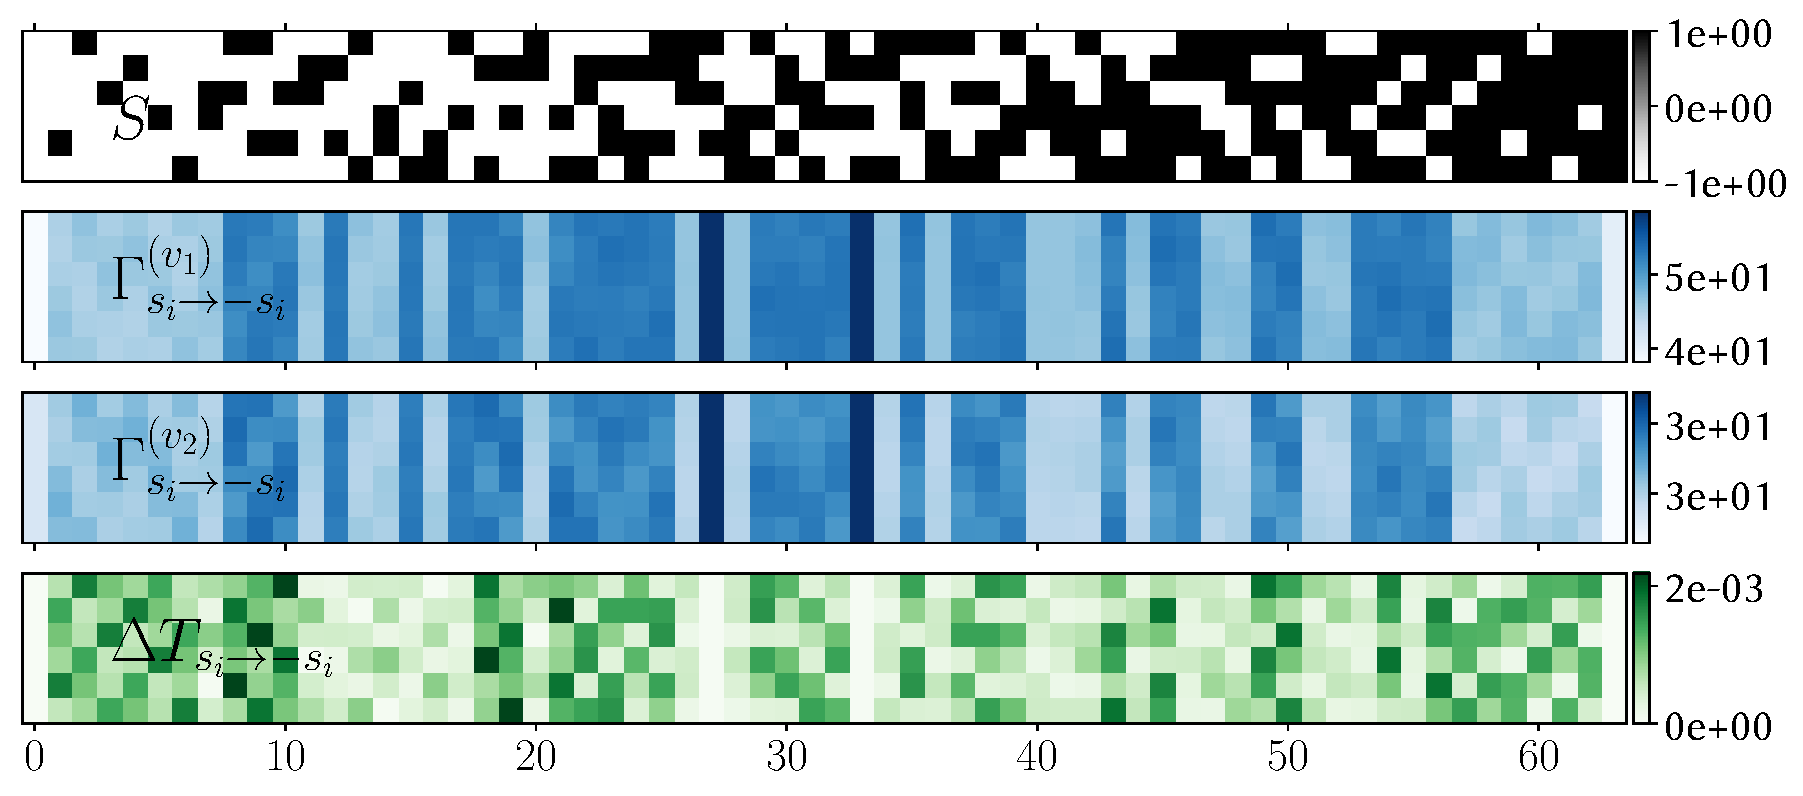
\includegraphics[width=\linewidth]{Chapter5/Figs/Vector/rate_structure.pdf}
	\caption[Structure of learned rates for 1D TFIM]{\textbf{Structure of rates in 1D TFIM.} Figure displays the underlying \emph{structure} learned in the 1d-TFIM ($L=6, J=1.0, h=1.0$) using the simple permutation batch. The optimal rates $\Gamma^{(v_1)}_{s_i \rightarrow -s_i}$, $\Gamma^{(v_2)}_{s_i \rightarrow -s_i}$ obtained with two initialisations (\textbf{middle}) for each configuration (\textbf{top}), look very similar. The jump matrices $T^{(v_1)}_{s_i \rightarrow -s_i}$, $T^{(v_2)}_{s_i \rightarrow -s_i}$ corresponding to the learned CTMCs are nearly the same (\textbf{bottom}), with maximum absolute difference being $\Delta_{\text{max}} T_{s_i \rightarrow -s_i} \approx 2\cdot10^{-3}$.}
	\label{fig:rate_structure}
\end{figure}

The issue in learning the timescale is not in the logarithm Radon-Nikodym loss, but in the way we generate batches. Moreover, this issue applies to a wider range of models than just the TFIM. For any model which has the following properties
\begin{enumerate}
	\item The passive rates are constant and the same for all adjacent states $\Gamma_{s \rightarrow s^{\prime}}=g$
	\item The number of adjacent states $N_a$ is independent for any state $s$
\end{enumerate}
it the $\log \text{RN}$ loss is \textbf{detached} from the passive rates $g$, if the variance is calculated from a batch of trajectories with same time $T$ and number of actions $N_{\text{actions}}$. Detached in this context means that the passive rates $g$ have no effect on the variance and hence on the optimisation of the rates. This can be seen by inserting 
\begin{equation}
	V(\mathrm{s})=-\sum_{s \neq s^{\prime}} \Gamma_{s \rightarrow s^{\prime}}+H_{s s}=-g N_a + H_{s s} \quad \text{ and } \quad \Gamma_{s \rightarrow s^{\prime}}=g
\end{equation}
into
\begin{equation}
	\begin{aligned}
			{\operatorname{Var}}\Bigg[\int\bigg(V(k(t))+&\sum_{l \neq k(t)}\bigg(\Gamma_{k(t) \rightarrow l}-\Gamma_{k(t) \rightarrow l}^{(v)}\bigg)\bigg) \mathrm{d} t \\
		&+\sum_{n} \log \left(\frac{\Gamma_{k^{(n)} \rightarrow k^{(n+1)}}^{(v)}}{\Gamma_{k^{(n)} \rightarrow k^{(n+1)}}}\right)-E_{0} T-\log \left(\frac{\varphi(k^{(N)})}{\varphi(k^{(0)})}\right)
		\Bigg],
	\end{aligned}
\end{equation}
to obtain
\begin{equation}
	\begin{aligned}
		\operatorname{Var}\Bigg[\int\left(H_{s s}-\sum_{l \neq k(t)}\Gamma_{k(t) \rightarrow l}^{(v)}\right)\mathrm{d} t 
		&+ \sum_{n} \log \left(\Gamma_{k^{(n)} \rightarrow k^{(n+1)}}^{(v)}\right)\Bigg] \\ &-E_{0} T -\log \left(\frac{\varphi(k^{(N)})}{\varphi(k^{(0)})}\right) \textcolor{red}{- gN_aT + gN_aT - N_{\text{actions}}\log{(g)}}.
	\end{aligned}
\end{equation}
The terms in red contain the passive rates, and can be taken out of $\operatorname{Var}[\cdot]$. The TFIM obeys both listed properties, and a \emph{permute} batch has constant $T$ and $N_{\text{actions}}$, meaning that we find ourselves in a regime where the correct timescale $\lambda$ \textbf{cannot} be learned. 

\subsection{Alternative Batch generation}
Unlearnable timescale for the \emph{permute} batch puts us in a precarious situation. The only way forward in models with the timescale learning issue is to work with trajectories of different lengths $N_{\text{actions}}$, fixed endpoints, and fixed time\footnote{Otherwise we cannot neglect $E_0T$ term.} $T$. This is computationally disadvantageous, because we can no longer evaluate $\log \text{RN}$ on the whole batch in parallel. Moreover, the generation of the batch becomes difficult to implement and may become a bottleneck itself. 

We test the \emph{construct} batch, an alternative batch generation technique described in section~\ref{sec:qoptsampl}. 
\begin{figure}[h]
	\centering
	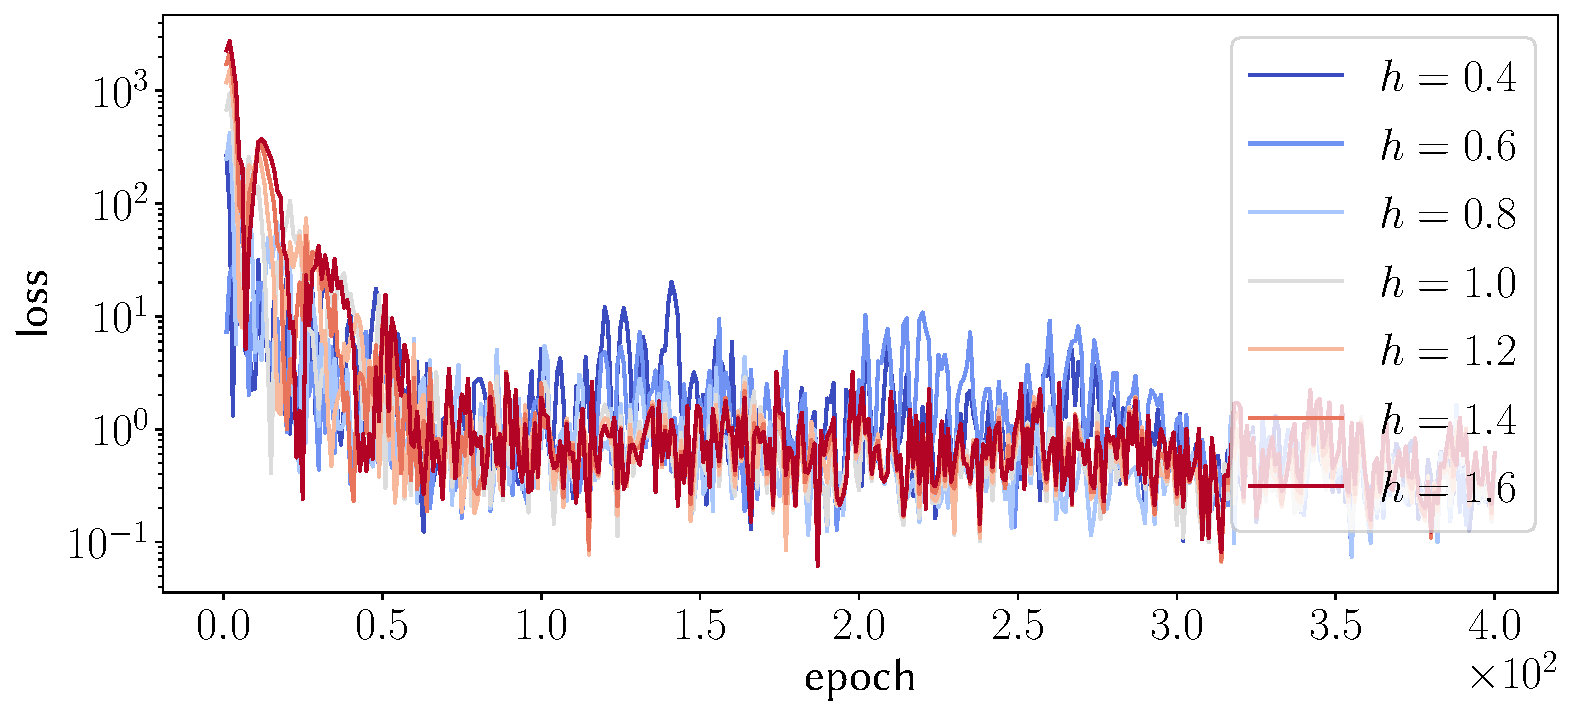
\includegraphics[width=\linewidth]{Chapter5/Figs/Vector/constr-g-loss}
	\caption[Rate training in 1d-TFIM using the \emph{construct} method]{\textbf{Rate training in 1d-TFIM using the construct method}. Optimisation with the \emph{construct} batch method, converges for different values of parameter $h$, moreover the obtained rates are not independent of $h$. Solved with $L=6, N_a=4, N_e=2, T=1$.}
	\label{fig:constr-g-loss}
\end{figure}
Fig.~\ref{fig:constr-g-loss} displays the training loss for the TFIM with different values of $h$ when using the \emph{construct} method for batch generation. Two things are apparent when optimising this new loss. First, it is even more volatile and increasing the batch size helps less than with the \emph{permute} batch. Second, the optimisation becomes more difficult when $h$ is smaller. It is also clear, that this loss now has the capability to scale the outputs of the model throughout optimisation, and at least for small times $T$ the timescale of the model is close to the passive timescale $\lambda_0$. This is clearly seen in Fig.~\ref{fig:troub}, where distributions of holding times are shown for a range of optimisation settings. 
\begin{figure}[H]
	\centering
	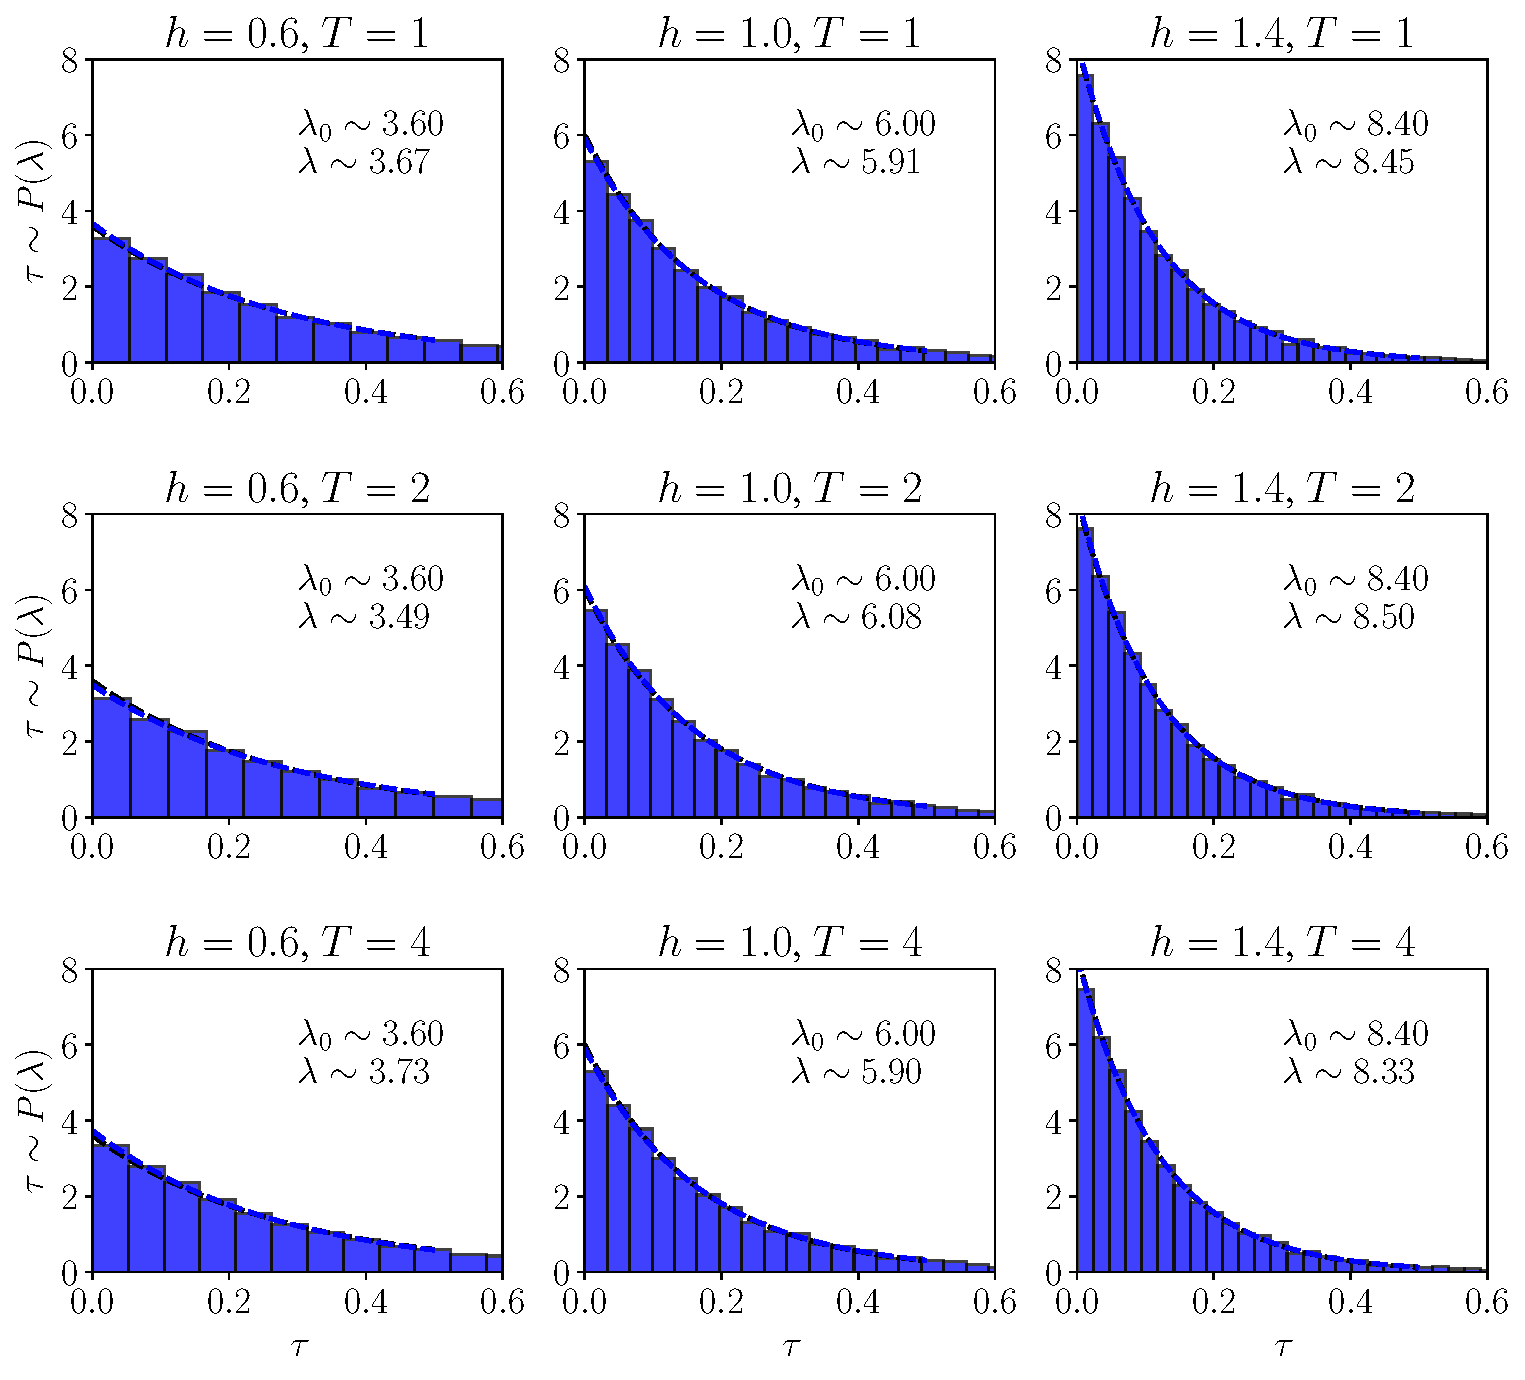
\includegraphics[width=1\linewidth]{Chapter5/Figs/Vector/troub}
	\caption[Distributions of holding times $\tau$ in 1d-TFIM with \emph{construct} batch]{\textbf{Distributions of holding times $\tau$ in 1d-TFIM with \emph{construct} batch.} The $\log\text{RN}$ loss is no longer decoupled from the rates, we see that the timescale $\lambda$ is learned by the model and is comparable to the passive rates $\lambda_0=hL$ for range of setups ($T$, $h$, $L=6$).}
	\label{fig:troub}
\end{figure}



\begin{figure}
	\centering
	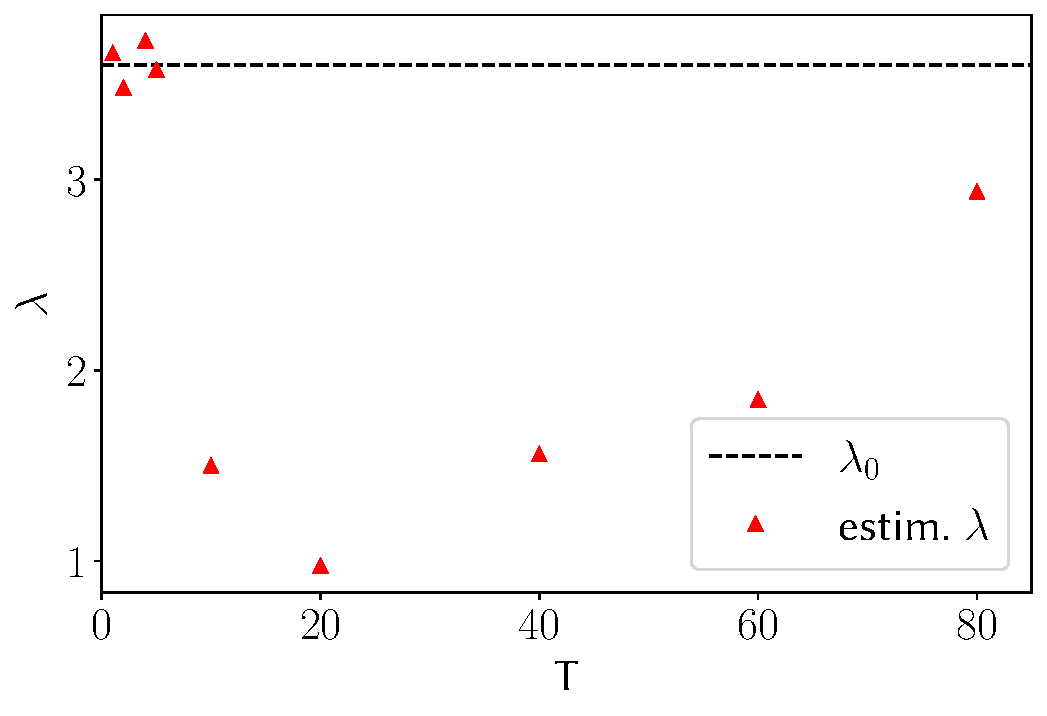
\includegraphics[width=0.5\linewidth]{Chapter5/Figs/Vector/Tvlamb}
	\caption[Timescale gap for the \emph{construct} batch.]{\textbf{Timescale gap for the \emph{construct} batch.} }
	\label{fig:tvlamb}
\end{figure}


\begin{figure}
	\centering
	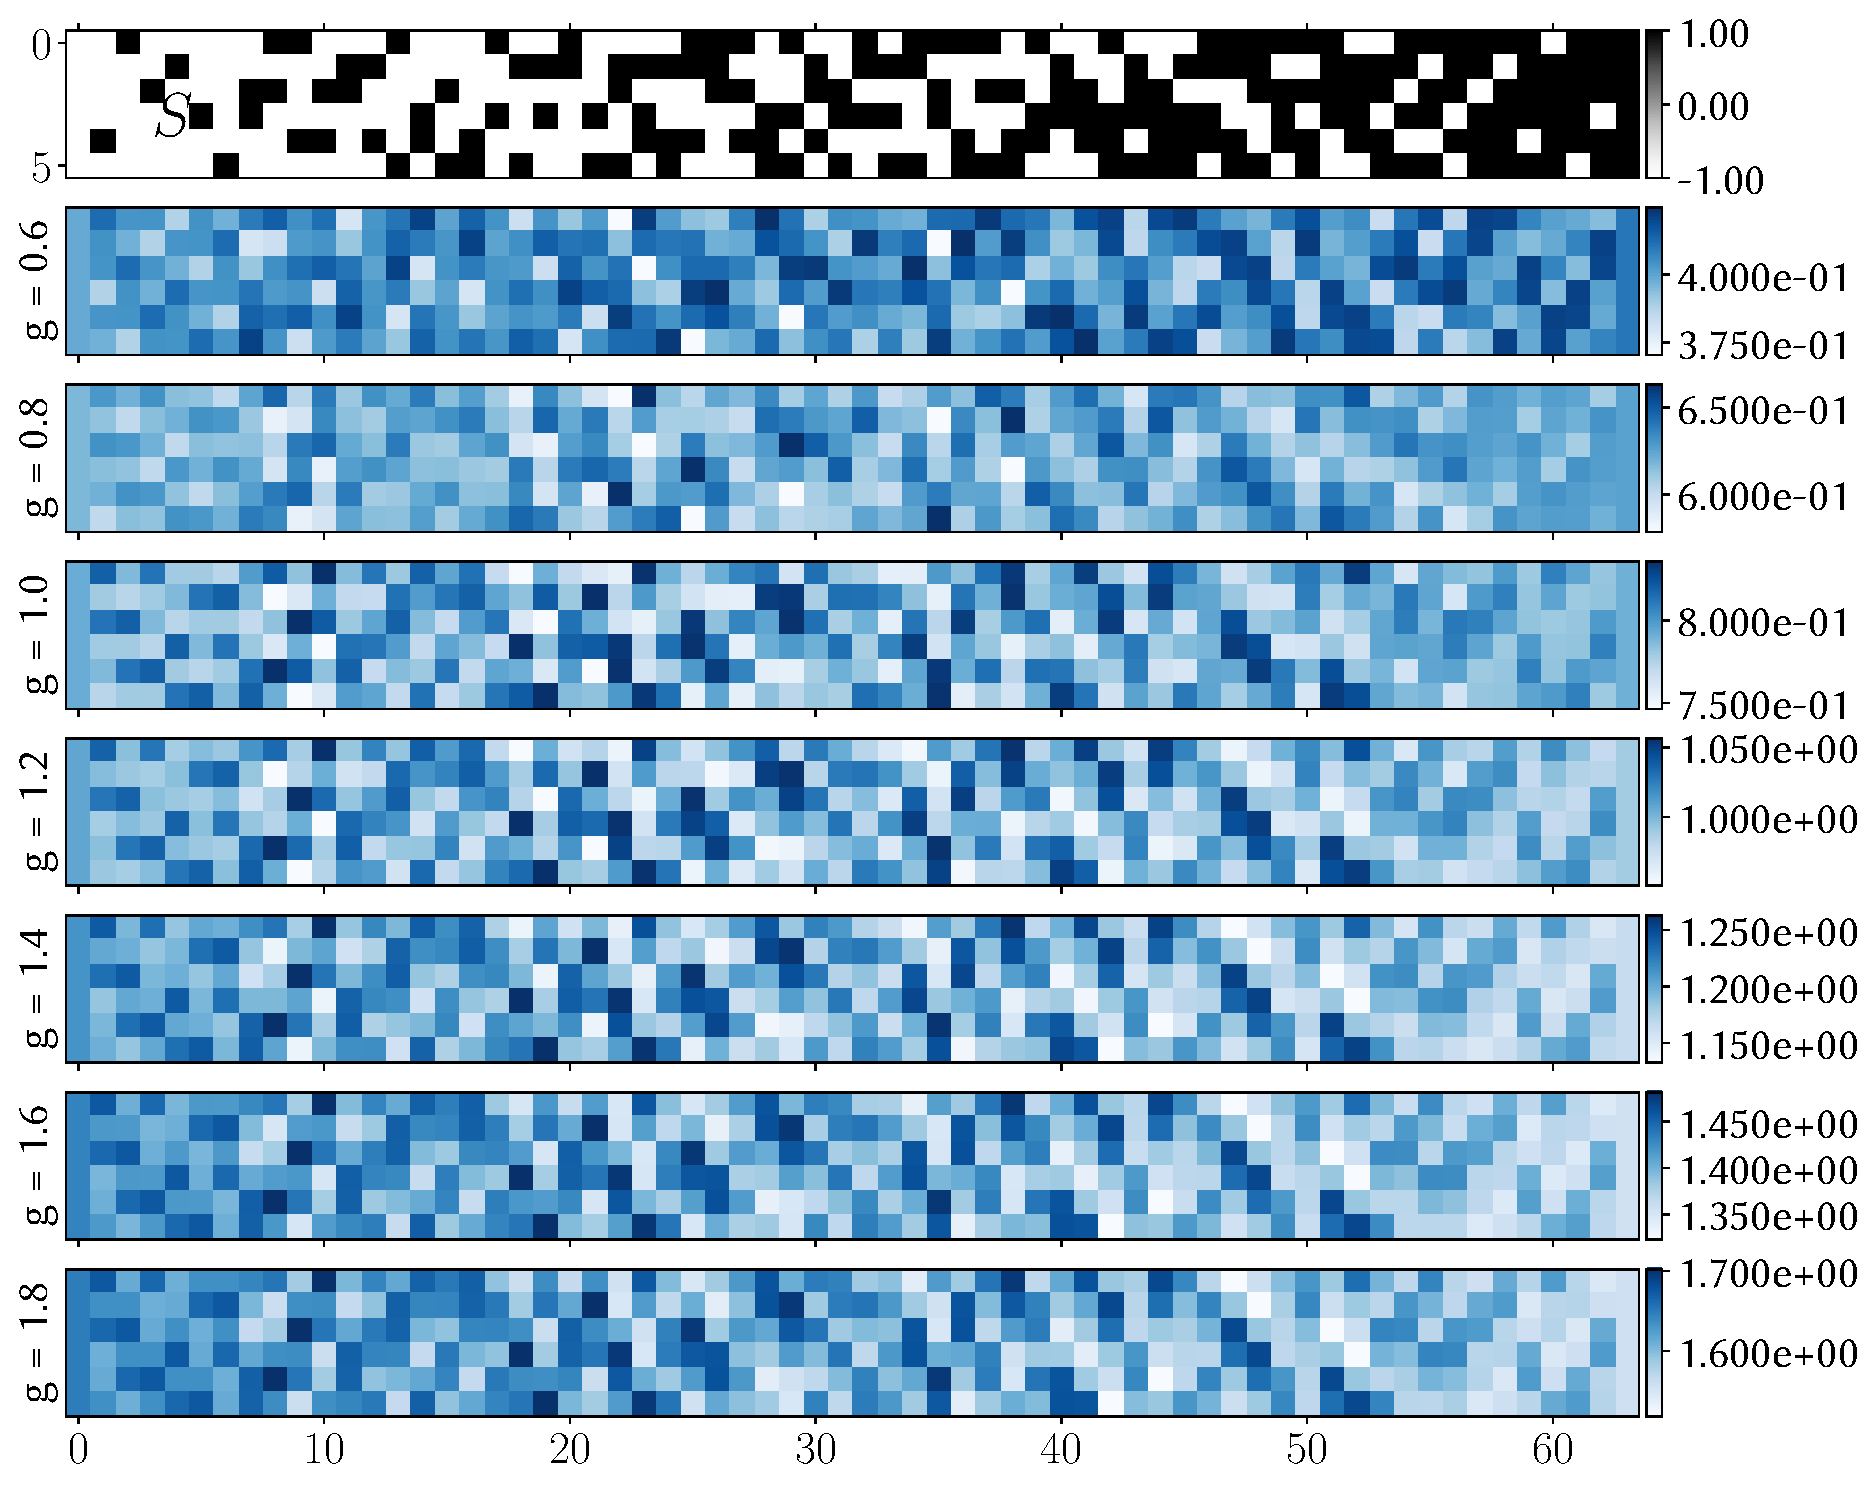
\includegraphics[width=1\linewidth]{Chapter5/Figs/Vector/troub_rates}
	\caption[Learned rates of the 1-dTFIM with the \emph{construct} batch]{\textbf{Learned rates of the 1-dTFIM with the \emph{construct} batch.}}
	\label{fig:troubrates}
\end{figure}

\begin{figure}
	\centering
	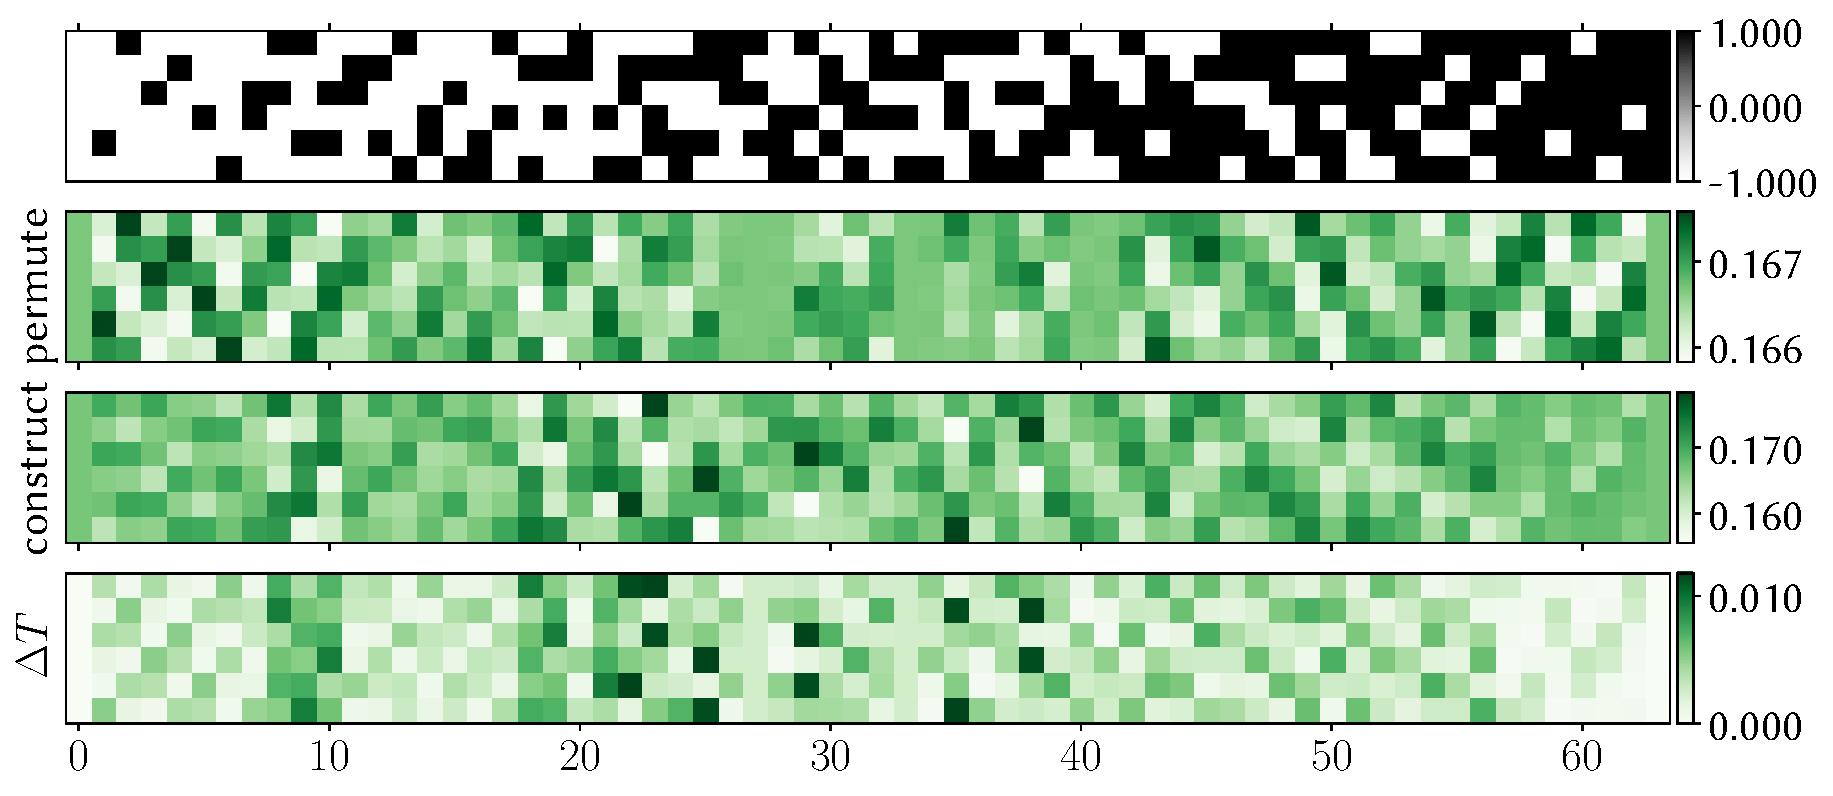
\includegraphics[width=1\linewidth]{Chapter5/Figs/Vector/rate_compare1}
	\caption[Comparison of \emph{jump matrices} $T$ for different batch types]{\textbf{Comparison of \emph{jump matrices} $T$ for different batch types.}}
	\label{fig:ratecompare1}
\end{figure}

\begin{figure}
	\centering
	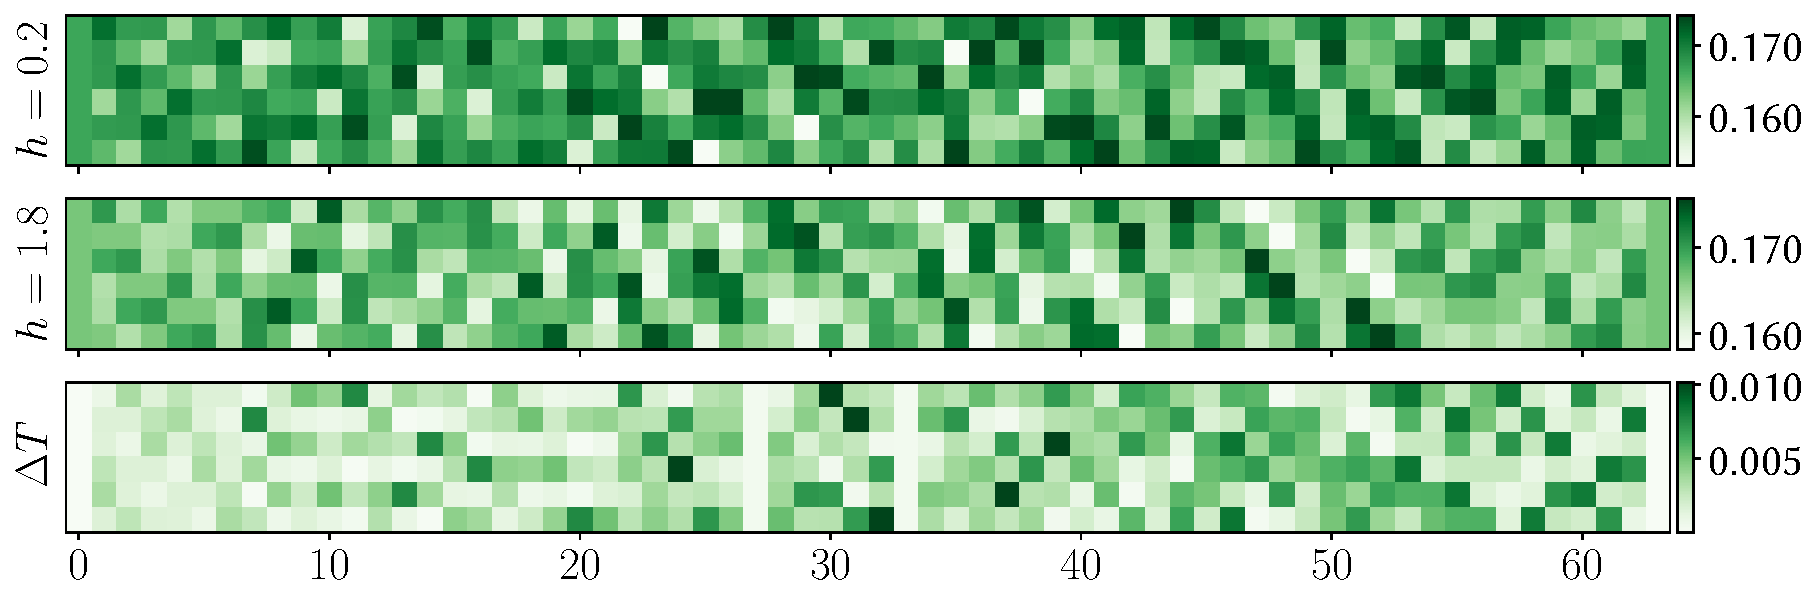
\includegraphics[width=1\linewidth]{Chapter5/Figs/Vector/rate_compare2}
	\caption[Comparison of \emph{jump matrices} $T$ for different batch types]{\textbf{Comparison of \emph{jump matrices} $T$ for different $h$.}}
	\label{fig:ratecompare2}
\end{figure}


\newpage
\subsection{Architectural choices}
\subsubsection{The pCNN}
As expected architecture choices and hyperparameters play an important role in learning the rates $\Gamma^{(v)}$, however how each separate parameter impacts the optimisation process is not very surprising, more interesting is perhaps the relative importance we can assign to each hyperparameter when compared to others. As we will see the hyperparameters play one of two roles. The CTMC simulation time $T$ and batch size $N_b$ stabilise the estimation of variance loss, thus improving the stability of the learning process and convergence, while the width $N_w$ of the pCNN and its depth $N_l$ increase the representational power of the NN.
\begin{figure}[H]
	\centering
	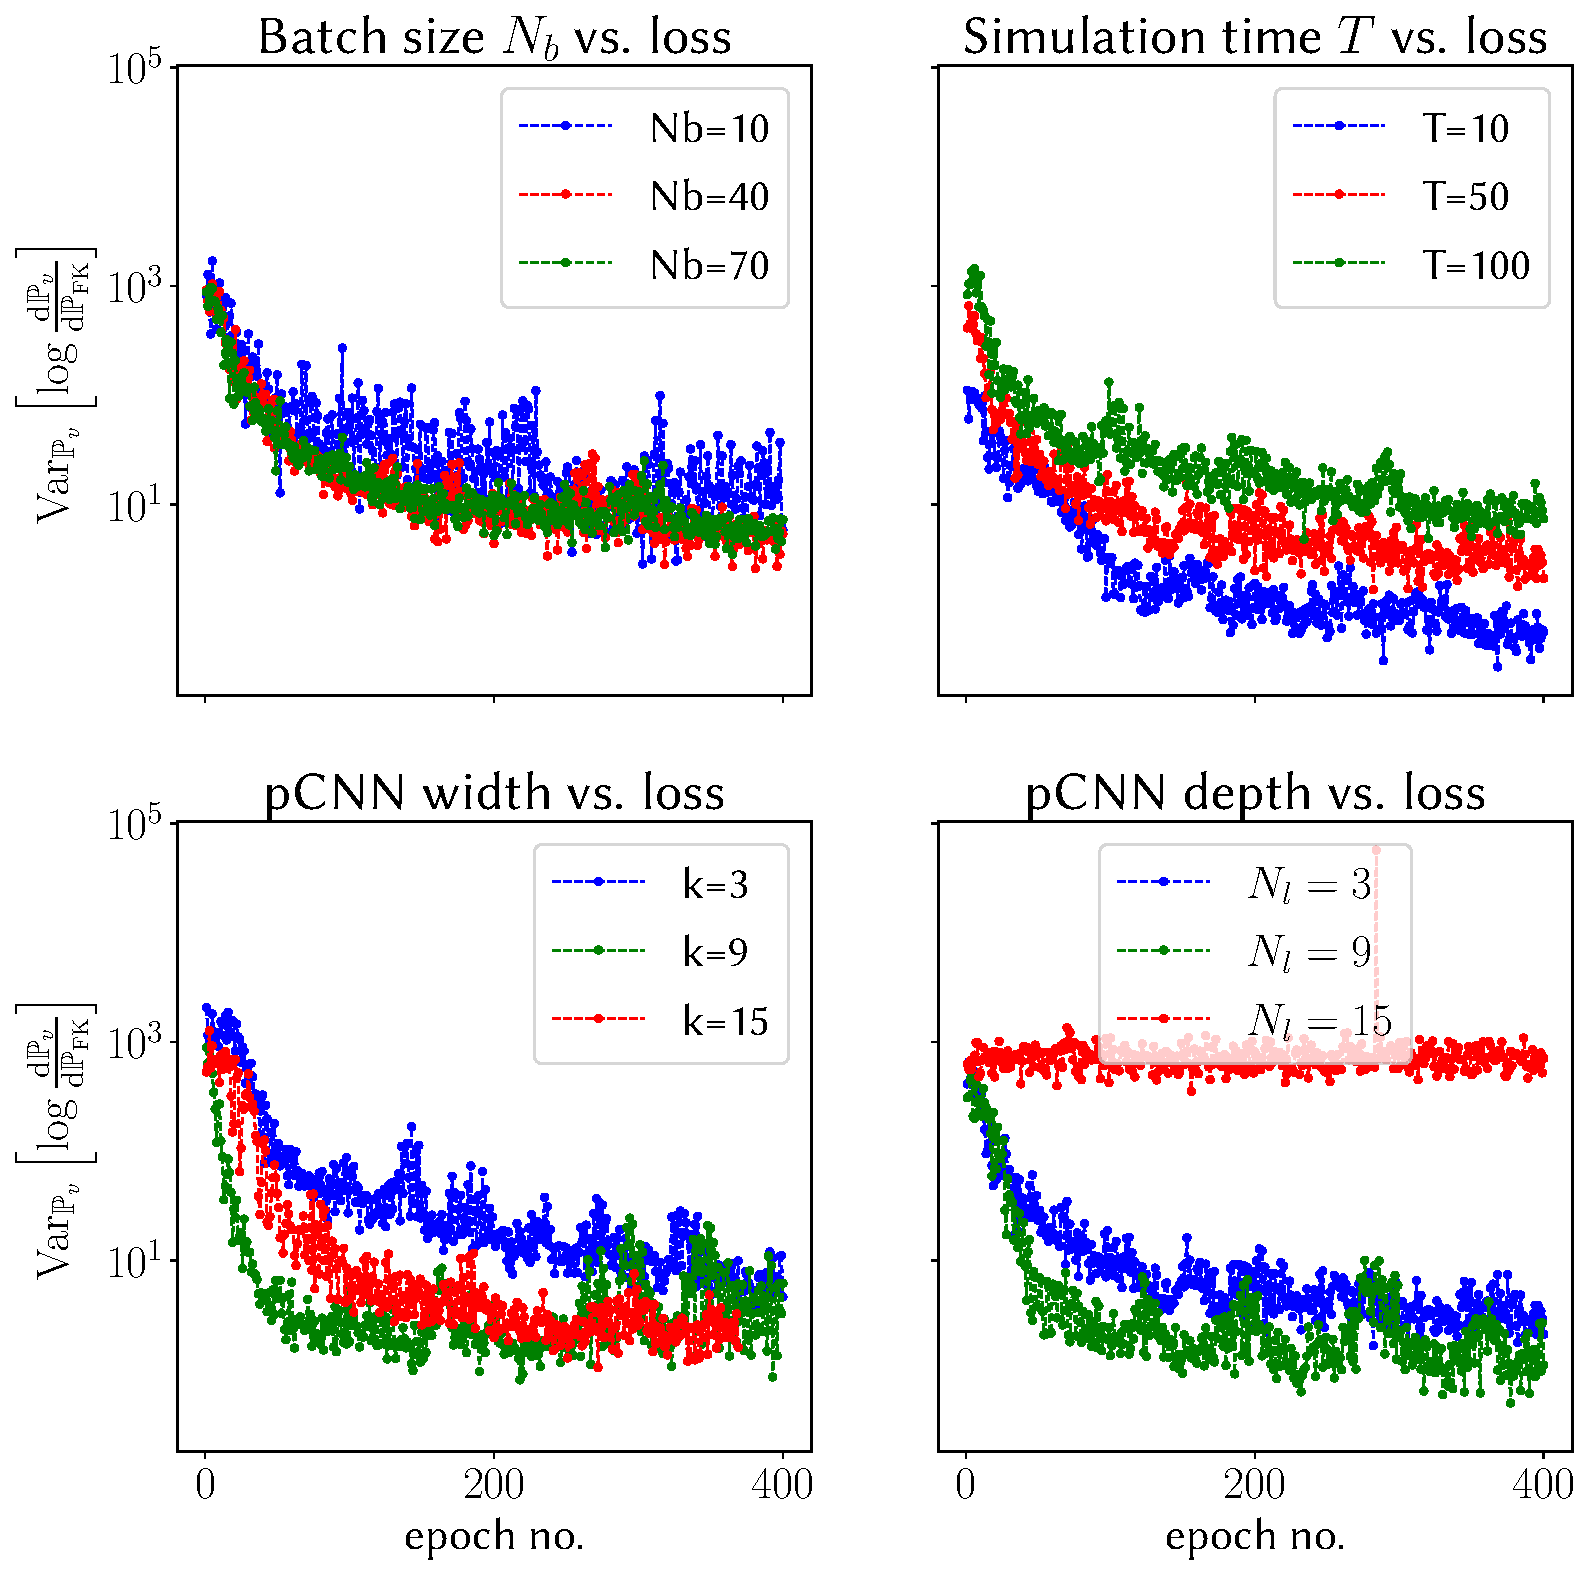
\includegraphics[width=\linewidth]{Chapter5/Figs/Vector/init_test_learning}
	\caption[Initial rate training experiments]{\textbf{Initial rate training experiments}. Learning experiments using \emph{initial} sampling mode and different simulation setups for 2d-TFIM ($L=3, J=1.0, h=1.0$). \textbf{top left:} $T = 75, N_w = 5, N_l = 3$, \textbf{top right:} $N_b = 50, N_w = 5, N_l = 3$, \textbf{bottom left:} $N_b = 50, T = 50, N_l = 3$, \textbf{bottom right:} $N_b = 50, T = 50, N_w = 5$.}
	\label{fig:inittestlearning}
\end{figure}
Initial experiments are shown in Fig.~\ref{fig:inittestlearning}, the top row displays the aforementioned stability. Increasing the batch size decreases the "volatility" of the loss, and same is true for $T$, but only if we consider loss normalized per time unit. As a rule of thumb $N_w$ and $N_l$ do not have a significant impact on the efficiency/speed of training, so long as both hyperparameters are chosen to be somewhere in the goldilocks zone, deep and narrow networks sometimes struggle to converge, bottom right Fig.~\ref{fig:inittestlearning}.

Going beyond the training itself, we need to evaluate the \emph{generalisation} of the rates. The worry is that training the rates at certain $T$ and $N_b$ could overfit and negatively impact sampling down the line, where the $T$ will be very different. To test this the rates were trained for various settings of $T, N_b, N_w, N_l$ and tested them by evaluating the loss at $T=50$, $N_b=50$, Fig.~\ref{fig:avgvarloss}. What we learn is that the rates do not overfit, average test loss is in the same order of magnitude than the train loss, and that $N_b$ is more important for stability than $T$. Finally, as we want to construct the most effective ansatz for eventual sampling experiments, we also investigate the relative time and size cost of increasing hyperparameters, the results are in Fig.~\ref{fig:initialtimespace}.

\begin{figure}[H]
	\centering
	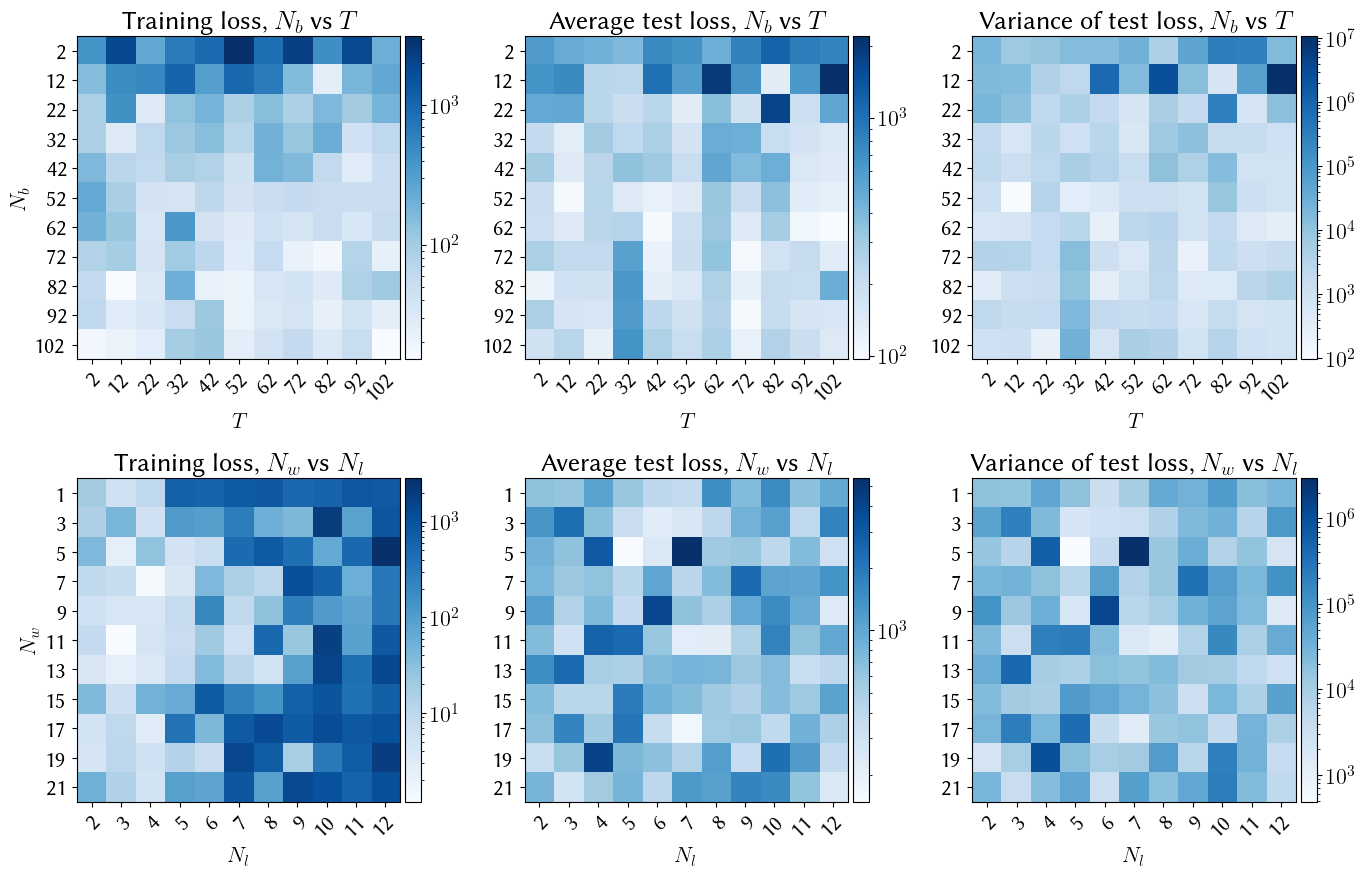
\includegraphics[width=\linewidth]{Chapter5/Figs/Raster/avg_var_loss}
	\caption[Generalisation capabilities of the pCNN]{\textbf{Generalisation capabilities of the pCNN.} Figure displays the effect of $T, N_b$ and $N_w, N_l$ on transferability of the learned rates using initial sampling, 2d-TFIM (L=3, J=1.0, h=1.0). Data was obtained by training the rates for different setups, sampling $N=15$ trajectories with $T=50$ from the learned rates for each setup, permuting the trajectories to obtain batches of $N_b=50$ and finally evaluating the average and sample variance of the $\log \text{RN}$ loss. Subfigures show (left to right) the loss after final epoch of training, average test loss, and variance of test loss. Setups: varying $N_b$ and $T$ at $N_w=3$, $N_l=3$ (\textbf{top}), varying $N_w$ and $N_l$ at $N_b=32$ and $T=30$ (\textbf{bottom}). All loss values are $T$ normalised.}
	\label{fig:avgvarloss}
\end{figure}

\begin{figure}[H]
	\centering
	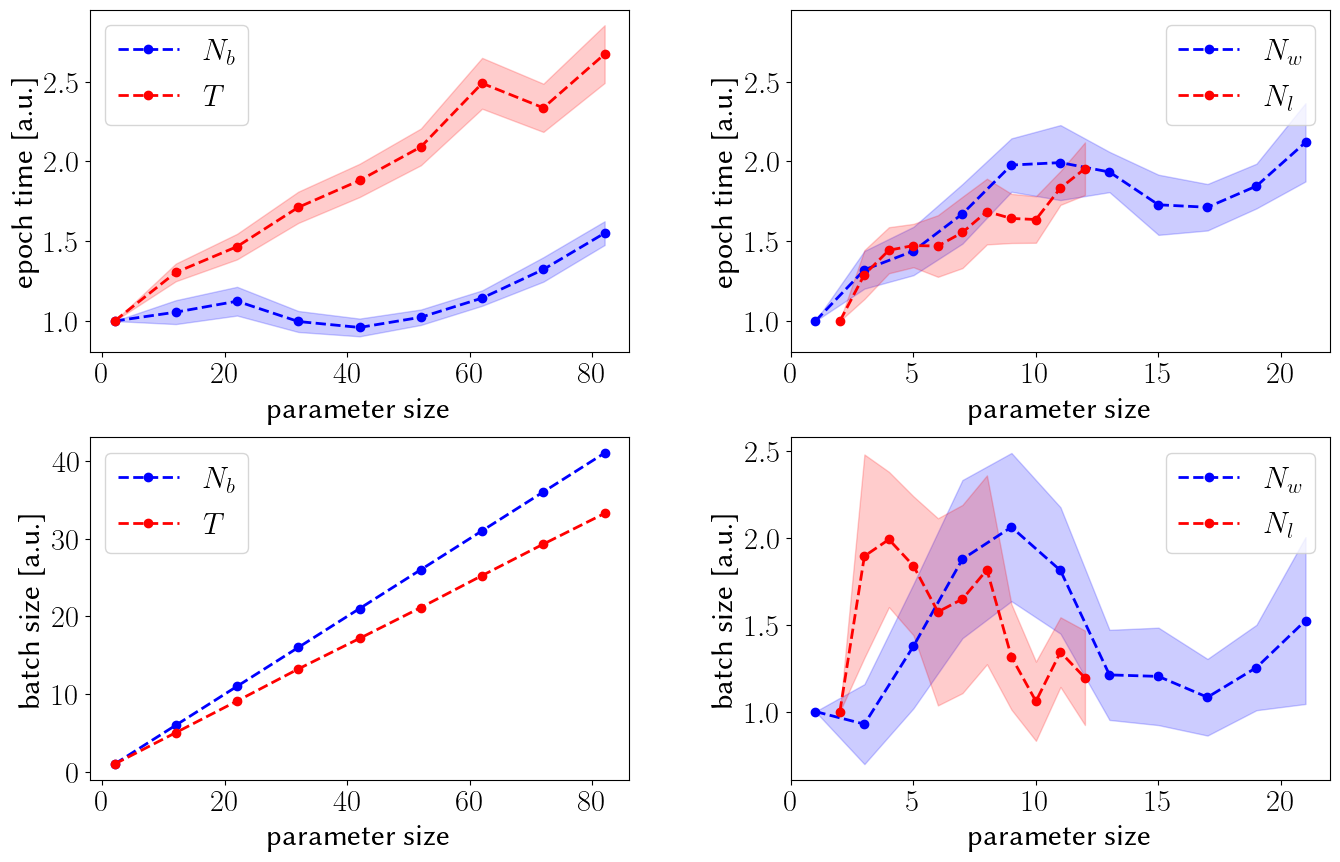
\includegraphics[width=\linewidth]{Chapter5/Figs/Raster/initial_time_space}
	\caption[Time and space complexity of the pCNN]{\textbf{Time and space complexity of the pCNN.} Comparison of normalised time needed per epoch averaged over $N=15$ samples, for different $T$, $N_b$ (\textbf{top left}) and $N_w$, $N_l$ (\textbf{top right}). Comparison of normalised batch size averaged over $N=15$ samples, for different $T$, $N_b$ (\textbf{bottom left}) and $N_w$, $N_l$ (\textbf{bottom right}). All values obtained from the same simulations as in Fig.~\ref{fig:avgvarloss}.}
	\label{fig:initialtimespace}
\end{figure}

\subsubsection{Comparison with G-pCNN}
A strong inductive bias, e.g. equivariance to translation or other appropriate symmetries should provide an advantage when learning a mapping equivariant to these same symmetries. Moreover, we expect this advantage to be even more significant in the case of learning with the $\log \text{RN}$ loss. This is because variational rates $\Gamma^{(v)}$ are evaluated multiple times in succession to evaluate the logarithm Radon-Nikodym derivative on a single trajectory, and this is repeated for a whole batch of trajectories.  

Initial training experiments were conducted on the TFIM, comparing the learning of a fully connected network, and the pCNN in 1D, as well as both compared to the group-equivariant CNN in two dimensions. Qualitatively, there is little difference in the performance of the pCNN and the MLP in 1d, whereas the difference becomes more notable in 2d, where the gCNN seems to learn quickest, when comparing networks with comparable numbers of variational parameters. These experiments are limited in two ways. First, due to the stochastic nature of the loss it is hard to tell which architecture is performing better and statistical metrics are needed. Second, because of a suboptimal implementation of the gCNN, runs with many epochs could not be carried out and the results are thus not conclusive. Further investigation is needed to confirm these qualitative results, it is suggested as future work. 

\section{Importance sampling}

\subsection{Ising model}

\begin{figure}[H]
	\centering
	\subfloat[Original]{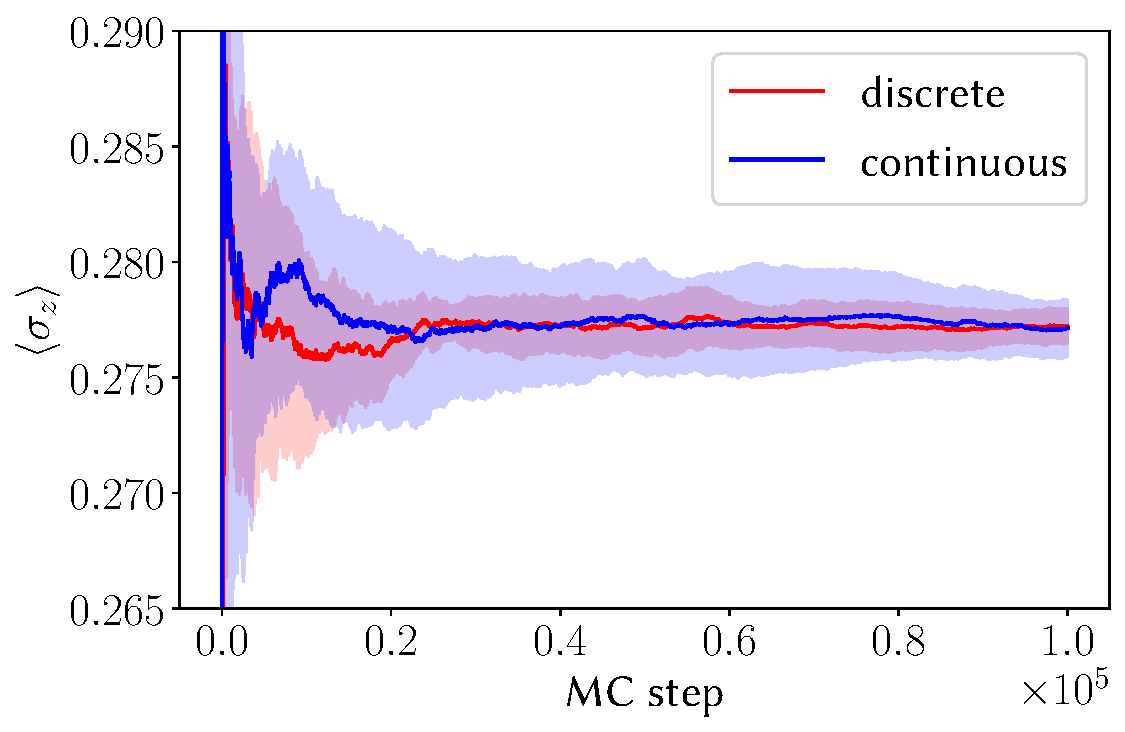
\includegraphics[width=0.45\linewidth]{Chapter5/Figs/Vector/sampling_example}}
	\quad
	\subfloat[Reparametrized]{	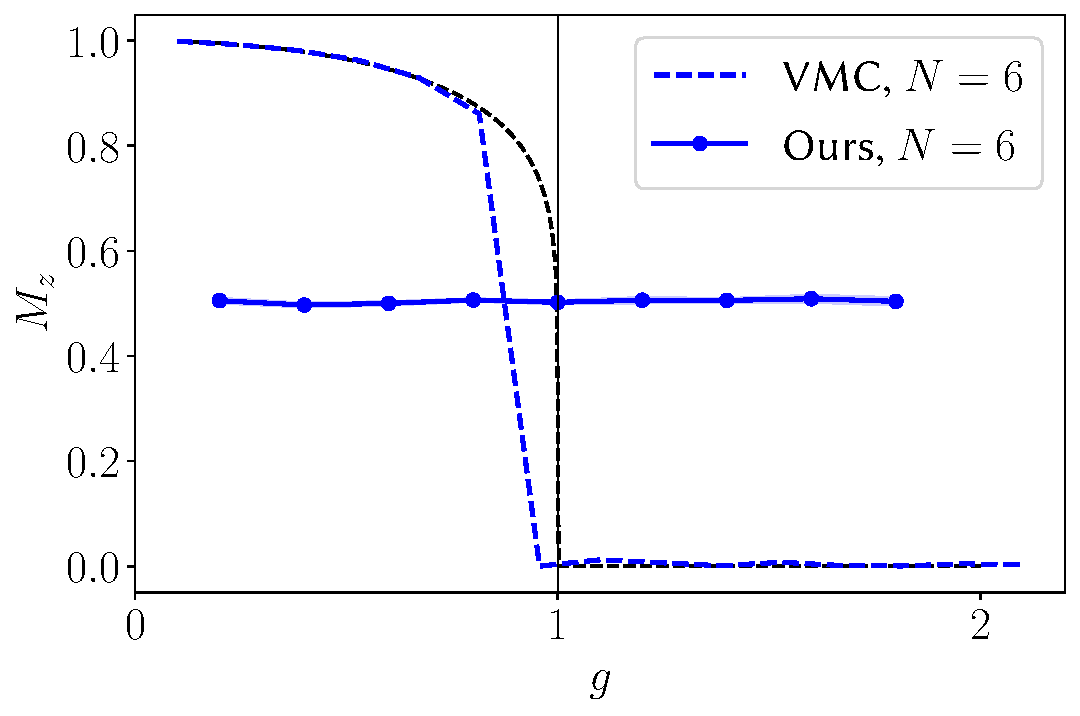
\includegraphics[width=0.45\linewidth]{Chapter5/Figs/Vector/tfim1d_finite_scaling-justsigz.pdf}}
	\caption[Sampling in the TFIM model]{\textbf{Sampling in the TFIM model}}
	\label{fig:sampling_tfim1d}
\end{figure}

